\documentclass[journal = jpccck, manuscript = suppinfo]{achemso}
\setkeys{acs}{usetitle = true}
\usepackage{fixltx2e}
\usepackage{float}
\usepackage{achemso}
\usepackage{natbib}
\usepackage{multirow}
\usepackage{wrapfig}
\usepackage{times}
\usepackage{tablefootnote}
\usepackage{booktabs}
\usepackage[version=3]{mhchem}  % this is a great package for formatting chemical reactions
\usepackage{url}

\mathchardef\mhyphen="2D

\title{Island formation on \ce{Pt}/\ce{Pd}(557) surface alloys in the presence
of adsorbed \ce{CO}: A molecular dynamics study}


\author{Joseph R. Michalka}
\author{J. Daniel Gezelter}
\email{gezelter@nd.edu}
\affiliation[University of Notre Dame]{251 Nieuwland Science Hall\\
  Department of Chemistry and Biochemistry\\ University of Notre
  Dame\\ Notre Dame, Indiana 46556}

\keywords{}

\begin{document}

The new \ce{Pd}-\ce{CO} potential energy function discussed in the
main text recovers the experimental $c(4 \times 2)$ surface structure
at high coverages.  In figure \ref{fig:C4x2}, we show that relatively
large domains of $c(4 \times 2)$ ordered \ce{CO} form on the surface.
The surface was prepared as a perfect \ce{Pd}(111) at 500~K, and was
dosed with a 0.5 ML coverage of gas phase \ce{CO}.  The system was
then cooled from 500~K to 130~K over 2~ns.  The domains and incomplete
ordering are a result of the rapid cooling.

\begin{figure}
  \includegraphics[width=\linewidth]{../figures/SupportingInformation/C4x2_best.pdf}
  \caption{0.50 ML of \ce{CO} on a \ce{Pd}(111) surface adopts domains
    (outlined in cyan boundaries) of the $c(4 \times 2)$
    configuration. The surface started at 500~K and was cooled to
    130~K over 2~ns.  At this relatively high cooling rate, multiple
    domains with different orientations of the $c(4 \times 2)$ pattern
    are displayed.}
\label{fig:C4x2}
\end{figure}

\newpage

The newly-fit \ce{Pt}-\ce{CO} potential energy function discussed in
the main text recovers the experimental
$(\sqrt{3} \times \sqrt{3}) R~30^{\circ}$ surface structure at a 1/3
ML coverage.  In figure \ref{fig:Root3}, we show that small domains of
$(\sqrt{3} \times \sqrt{3}) R~30^{\circ}$ ordered \ce{CO} form on the
surface.  The surface was prepared as a perfect \ce{Pt}(111) at 500~K,
and was dosed with a 0.33 ML coverage of gas phase \ce{CO}.  The
system was then cooled from 500~K to 130~K over 10~ns.  The small
domains and incomplete ordering are a result of the relatively rapid
cooling.

\begin{figure}
  \includegraphics[width=\linewidth]{../figures/SupportingInformation/Pt_33_root3.pdf}
  \caption{0.33 ML of \ce{CO} on a \ce{Pt}(111) surface adopts domains
    (outlined in cyan boundaries) of the
    $(\sqrt{3} \times \sqrt{3}) R~30^{\circ}$ configuration. The
    surface started at 500~K and was cooled to 130~K over 10~ns.  At
    this cooling rate, small domains with different orientations of
    the $(\sqrt{3} \times \sqrt{3}) R~30^{\circ}$ pattern are
    displayed.}
\label{fig:Root3}
\end{figure}

\newpage

An expanded version of figure 3 in the main text which contains data
for all five \ce{CO} coverage levels.

\begin{figure}
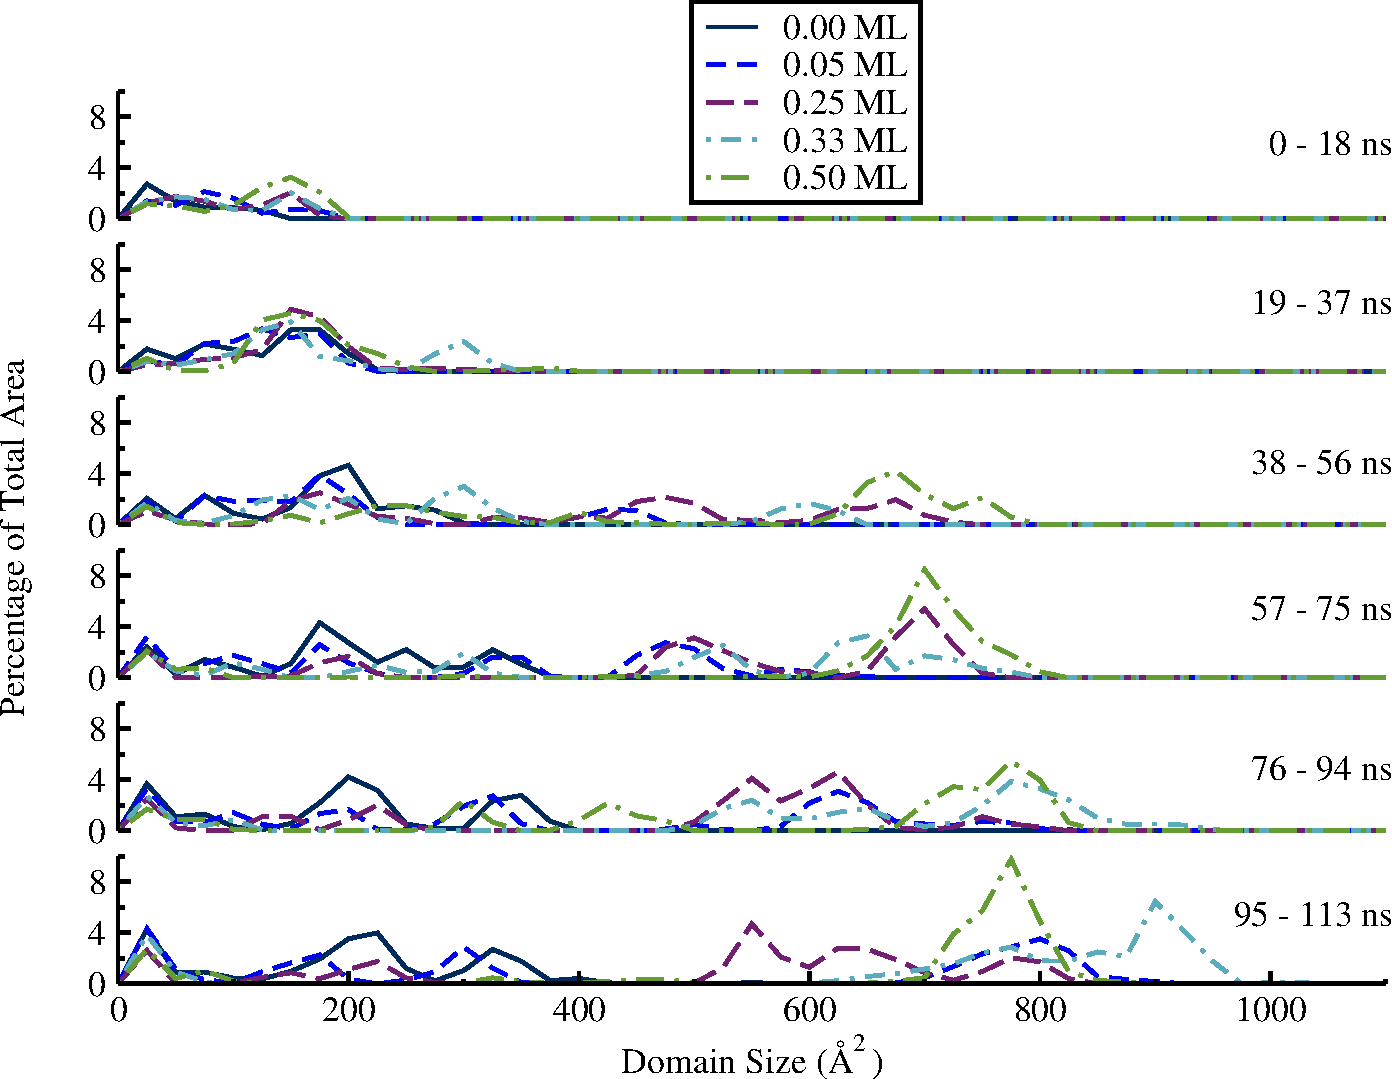
\includegraphics[width=\linewidth]{../figures/SupportingInformation/domainSize_Pd_SI.pdf}
\caption{Distributions of \ce{Pd} domain sizes at all simulated
\ce{CO} coverages at different times after exposure to \ce{CO}.}
\label{fig:Pd_SI}
\end{figure}

\newpage

An expanded version of figure 4 in the main text which contains data
for all five \ce{CO} coverage levels.

\begin{figure}
  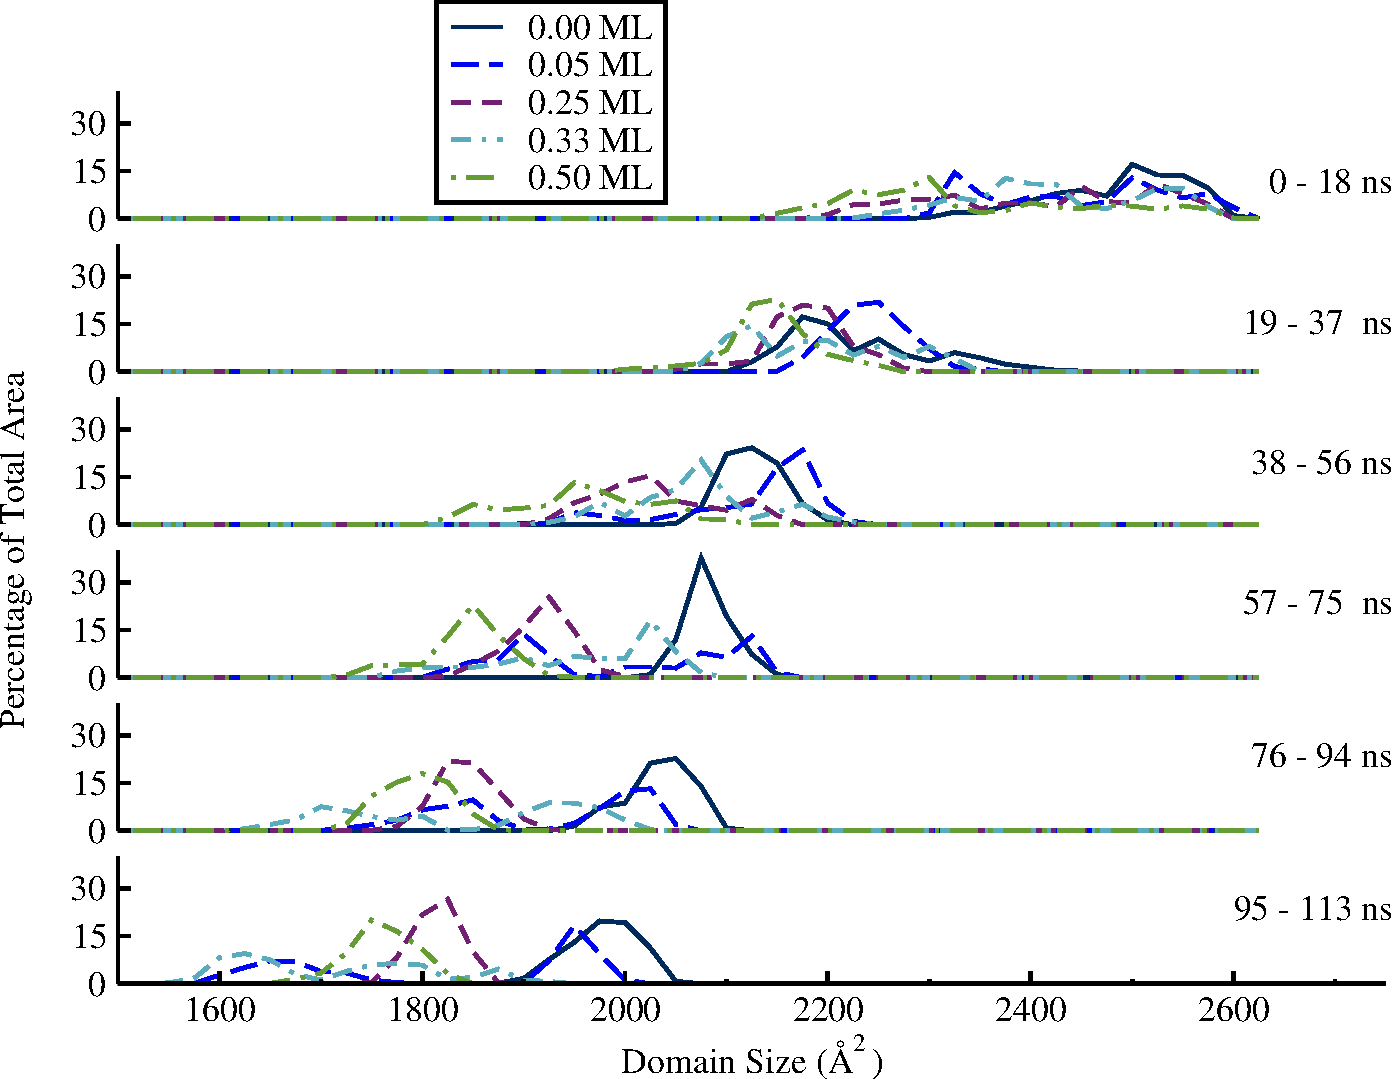
\includegraphics[width=\linewidth]{../figures/SupportingInformation/domainSizes_Pt_SI_zoomed.pdf}
  \caption{Distribution of large \ce{Pt} domain sizes at all simulated
    \ce{CO} coverages at different times after exposure to \ce{CO}.}
\label{fig:Pt_SI_big}
\end{figure}

\newpage

Figure \ref{fig:Pt_SI_small} contains data on the \ce{Pt} domains that
were $<$ 100 \AA\textsuperscript{2} in area.  Typical domains with
larger surface areas typically comprise 15-20\% of the total area,
while these smaller domains never reach 1\% of the total. These
domains correspond to 1-to-2 atom clusters of \ce{Pt} that exist
surrounded by \ce{Pd}. This situation can arise either from \ce{Pt}
adatom movement over the \ce{Pd} surface, or \ce{Pt}-\ce{Pd}
inversion.

\begin{figure}
  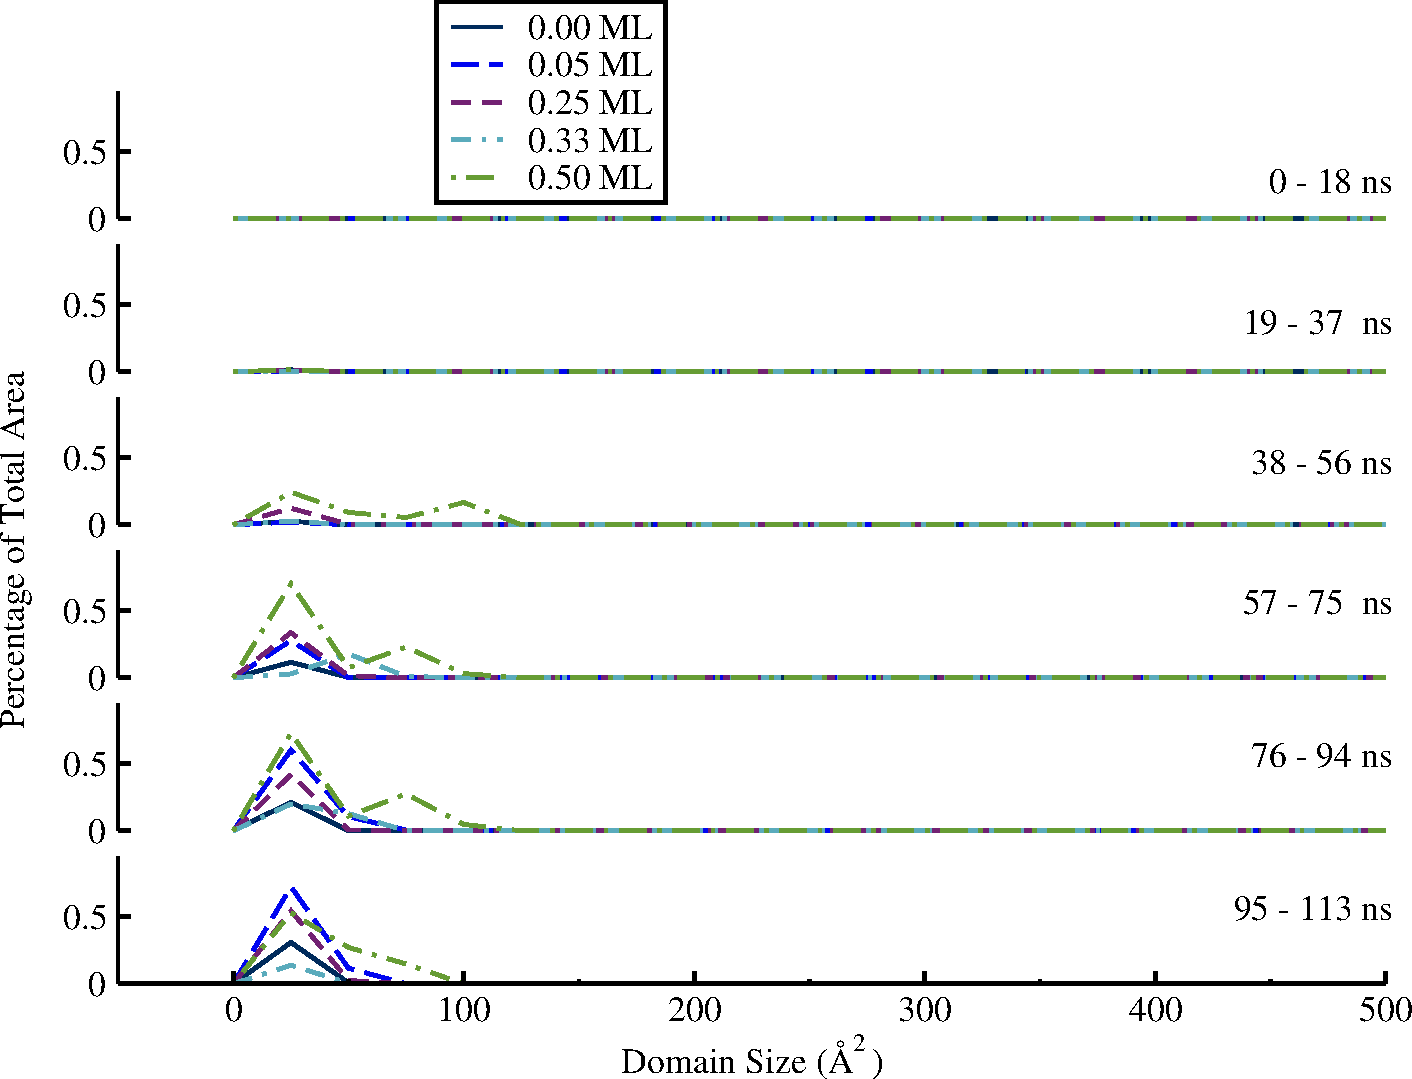
\includegraphics[width=\linewidth]{../figures/SupportingInformation/domainSizes_Pt_SI_smallFocus.pdf}
  \caption{Distribution of small \ce{Pt} domain sizes at different
    \ce{CO} coverages and at different times after exposure to
    \ce{CO}. Note that the $y$-axis is significantly smaller than in
    figure 4 in the main text.}
\label{fig:Pt_SI_small}
\end{figure}


\newpage

In the surface alloys, the reconstruction involves mostly \ce{Pt} atom
motion, leaving the underlying \ce{Pd}(557) substrate mostly intact.
This is easily seen when the \ce{Pt} atoms in the left image below are
hidden.  The small amount of step-wandering and step-breaking of the
underlying \ce{Pd} highlighted on the right side of fig. \ref{fig:557}
shows the strong tendency of \ce{Pd} to maintain the (557) steps.
Additionally, the main deviations of the \ce{Pd} substrate observed
here appear to be tied to the locations of islands in the \ce{Pt} top
layer.

\begin{figure}
  \includegraphics[width=\linewidth]{../figures/SupportingInformation/557.pdf}
  \caption{Snapshots of the \ce{Pt}/\ce{Pd} 0.33 ML system after
    $\sim$110~ns (\ce{CO} hidden). The right panel highlights the
    stability of the underlying (557) \ce{Pd} substrate after hiding
    the surface \ce{Pt} atoms. \ce{Pt} atoms are shown in gray and
    \ce{Pd} atoms are shown in pink.}
\label{fig:557}
\end{figure}

\newpage

An expanded version of figure 5 in the main text which contains data
for all five \ce{CO} coverage levels.  The ordering of the coverages
is fairly well maintained, although the 0.25 and 0.33 ML curves cross
at a number of points.

\begin{figure}
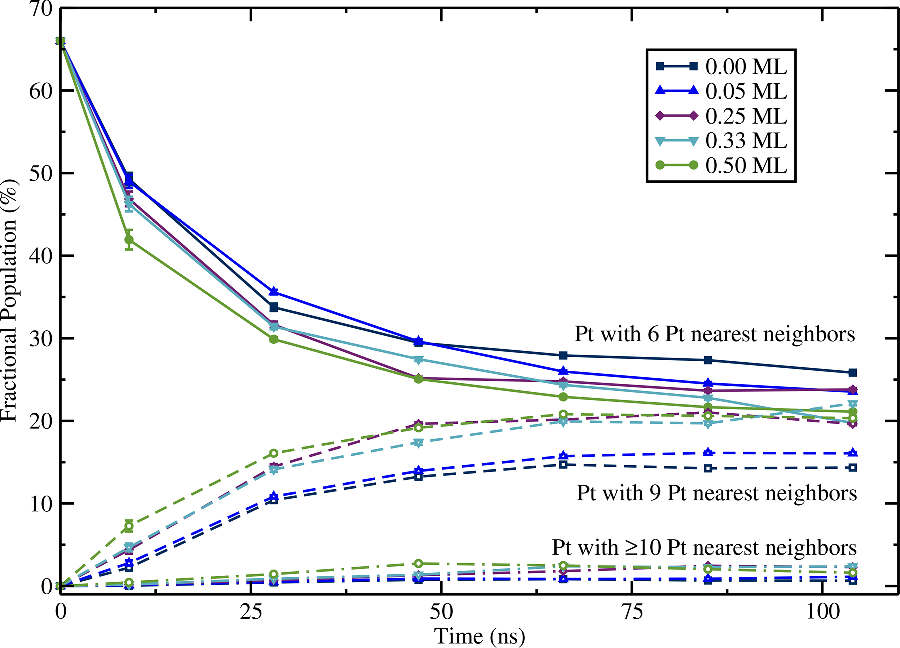
\includegraphics[width=\linewidth]{../figures/SupportingInformation/nearestNeighbor_full_withmorenn_photoshopped.pdf}
\caption{Population of \ce{Pt} atoms with either 6 (solid), 9
  (dashed), or $\ge$ 10 (dot-dashed) \ce{Pt} nearest neighbors
  averaged over 18~ns blocks of time.  At $t = 0$, the majority
  (2/3) of \ce{Pt} is located in the (111) plateaus where
  the number of \ce{Pt} nearest neighbors is 6. The remaining \ce{Pt}
  is located at step edges, with a neighbor \ce{Pt} count of 5.}
\label{fig:nn_full} 
\end{figure}

\newpage

\begin{acknowledgement}
  Support for this project was provided by the National Science
  Foundation under grant CHE-1362211 and by the Center for Sustainable
  Energy at Notre Dame (cSEND). Computational time was provided by the
  Center for Research Computing (CRC) at the University of Notre Dame.
\end{acknowledgement}


\end{document}



